\section{(n, 2) Tree Graph State}
\label{sec:n_2_tree}

Beginning from the final state derived from \cref{eq:tree_implementation}, by replicating the process outlined in \cref{eq:1_branch_implementation} to generate another branch, we could extend the implementation to create a generalized $(2, 2)$ tree graph state, thereby enabling the implementation of a $(n, 2)$ tree state.

As an example let us consider a $(3, 2)$ tree state (figure 1).
It can be implemented using the following sequence of gates.
\begin{equation}
    \begin{quantikz}[column sep=0.2cm]
      & \gate{Y_+} & \qw & \qw & \ctrl{1} & \qw & \qw & \qw & \qw & \qw & \qw & \ctrl{1} & \qw & \qw & \qw & \qw & \qw & \qw & \ctrl{1} & \qw & \qw & \qw  \\
      & \gate{Y_+} & \ctrl{3} & \gate{Y_-} & \control{} & \ctrl{2} & \gate{Y_+} & \swap{1} & \gate{Y_+} & \ctrl{6} & \gate{Y_-} & \control{} & \ctrl{5} & \gate{Y_+} & \swap{4} & \gate{Y_+} & \ctrl{8} & \gate{Y_-} & \control{} & \ctrl{7} & \gate{Y_+} & \qw  \\
      & \qw & \qw & \qw & \qw & \qw & \qw & \targX{} & \qw & \qw & \qw & \qw & \qw & \qw & \qw & \qw & \qw & \qw & \qw & \qw & \qw & \qw  \\
      & \qw & \qw & \qw & \qw & \targ{} & \qw & \qw & \qw & \qw & \qw & \qw & \qw & \qw & \qw & \qw & \qw & \qw & \qw & \qw & \qw & \qw  \\
      & \qw & \targ{} & \qw & \qw & \qw & \qw & \qw & \qw & \qw & \qw & \qw & \qw & \qw & \qw & \qw & \qw & \qw & \qw & \qw & \qw & \qw  \\
      & \qw & \qw & \qw & \qw & \qw & \qw & \qw & \qw & \qw & \qw & \qw & \qw & \qw & \targX{} & \qw & \qw & \qw & \qw & \qw & \qw & \qw  \\
      & \qw & \qw & \qw & \qw & \qw & \qw & \qw & \qw & \qw & \qw & \qw & \targ{} & \qw & \qw & \qw & \qw & \qw & \qw & \qw & \qw & \qw \\
      & \qw & \qw & \qw & \qw & \qw & \qw & \qw & \qw & \targ{} & \qw & \qw & \qw & \qw & \qw & \qw & \qw & \qw & \qw & \qw & \qw & \qw  \\
      & \qw & \qw & \qw & \qw & \qw & \qw & \qw & \qw & \qw & \qw & \qw & \qw & \qw & \qw & \qw & \qw & \qw & \qw & \targ{} & \qw & \qw  \\
      & \qw & \qw & \qw & \qw & \qw & \qw & \qw & \qw & \qw & \qw & \qw & \qw & \qw & \qw & \qw & \targ{} & \qw & \qw & \qw & \qw & \qw 
    \end{quantikz}
    \notag
\end{equation}

Although the initial state of all qubits in the protocol remains $\ket{0}$, for the sake of fitting the circuit within the page, we imply their initialization.

%\begin{figure}
%    \centering
%    

\tikzset{every picture/.style={line width=0.75pt}} %set default line width to 0.75pt        

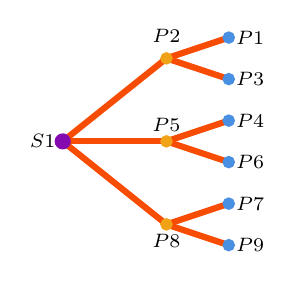
\begin{tikzpicture}[x=0.75pt,y=0.75pt,yscale=-1,xscale=1]
%uncomment if require: \path (0,182); %set diagram left start at 0, and has height of 182

%Straight Lines [id:da5808000645086375] 
\draw [color={rgb, 255:red, 246; green, 76; blue, 4 }  ,draw opacity=1 ][line width=2.25]    (360,70) -- (390,80) ;
%Straight Lines [id:da18975921226163972] 
\draw [color={rgb, 255:red, 246; green, 76; blue, 4 }  ,draw opacity=1 ][line width=2.25]    (390,60) -- (360,70) ;
%Straight Lines [id:da6595221878479601] 
\draw [color={rgb, 255:red, 246; green, 76; blue, 4 }  ,draw opacity=1 ][line width=2.25]    (360,110) -- (390,120) ;
%Straight Lines [id:da5683498370526975] 
\draw [color={rgb, 255:red, 246; green, 76; blue, 4 }  ,draw opacity=1 ][line width=2.25]    (390,100) -- (360,110) ;
%Straight Lines [id:da9165166451633462] 
\draw [color={rgb, 255:red, 246; green, 76; blue, 4 }  ,draw opacity=1 ][line width=2.25]    (360,30) -- (390,40) ;
%Straight Lines [id:da7926013585642647] 
\draw [color={rgb, 255:red, 246; green, 76; blue, 4 }  ,draw opacity=1 ][line width=2.25]    (390,20) -- (360,30) ;
%Straight Lines [id:da7417109803866969] 
\draw [color={rgb, 255:red, 246; green, 76; blue, 4 }  ,draw opacity=1 ][line width=2.25]    (310,70) -- (360,30) ;
%Straight Lines [id:da32862812153335397] 
\draw [color={rgb, 255:red, 246; green, 76; blue, 4 }  ,draw opacity=1 ][line width=2.25]    (310,70) -- (360,70) ;
%Straight Lines [id:da9935618987409959] 
\draw [color={rgb, 255:red, 246; green, 76; blue, 4 }  ,draw opacity=1 ][line width=2.25]    (310,70) -- (360,110) ;
%Shape: Circle [id:dp31789546772639043] 
\draw  [color={rgb, 255:red, 132; green, 9; blue, 175 }  ,draw opacity=1 ][fill={rgb, 255:red, 132; green, 9; blue, 175 }  ,fill opacity=1 ] (306.63,70) .. controls (306.63,68.14) and (308.14,66.63) .. (310,66.63) .. controls (311.86,66.63) and (313.38,68.14) .. (313.38,70) .. controls (313.38,71.86) and (311.86,73.38) .. (310,73.38) .. controls (308.14,73.38) and (306.63,71.86) .. (306.63,70) -- cycle ;
%Shape: Circle [id:dp6750291852439366] 
\draw  [color={rgb, 255:red, 74; green, 144; blue, 226 }  ,draw opacity=1 ][fill={rgb, 255:red, 74; green, 144; blue, 226 }  ,fill opacity=1 ] (387.5,120) .. controls (387.5,118.62) and (388.62,117.5) .. (390,117.5) .. controls (391.38,117.5) and (392.5,118.62) .. (392.5,120) .. controls (392.5,121.38) and (391.38,122.5) .. (390,122.5) .. controls (388.62,122.5) and (387.5,121.38) .. (387.5,120) -- cycle ;
%Shape: Circle [id:dp5494552717190384] 
\draw  [color={rgb, 255:red, 241; green, 163; blue, 23 }  ,draw opacity=1 ][fill={rgb, 255:red, 241; green, 163; blue, 23 }  ,fill opacity=1 ] (357.5,110) .. controls (357.5,108.62) and (358.62,107.5) .. (360,107.5) .. controls (361.38,107.5) and (362.5,108.62) .. (362.5,110) .. controls (362.5,111.38) and (361.38,112.5) .. (360,112.5) .. controls (358.62,112.5) and (357.5,111.38) .. (357.5,110) -- cycle ;
%Shape: Circle [id:dp8629159729730512] 
\draw  [color={rgb, 255:red, 74; green, 144; blue, 226 }  ,draw opacity=1 ][fill={rgb, 255:red, 74; green, 144; blue, 226 }  ,fill opacity=1 ] (387.5,80) .. controls (387.5,78.62) and (388.62,77.5) .. (390,77.5) .. controls (391.38,77.5) and (392.5,78.62) .. (392.5,80) .. controls (392.5,81.38) and (391.38,82.5) .. (390,82.5) .. controls (388.62,82.5) and (387.5,81.38) .. (387.5,80) -- cycle ;
%Shape: Circle [id:dp6642418585732942] 
\draw  [color={rgb, 255:red, 241; green, 163; blue, 23 }  ,draw opacity=1 ][fill={rgb, 255:red, 241; green, 163; blue, 23 }  ,fill opacity=1 ] (357.5,70) .. controls (357.5,68.62) and (358.62,67.5) .. (360,67.5) .. controls (361.38,67.5) and (362.5,68.62) .. (362.5,70) .. controls (362.5,71.38) and (361.38,72.5) .. (360,72.5) .. controls (358.62,72.5) and (357.5,71.38) .. (357.5,70) -- cycle ;
%Shape: Circle [id:dp6409499135433837] 
\draw  [color={rgb, 255:red, 74; green, 144; blue, 226 }  ,draw opacity=1 ][fill={rgb, 255:red, 74; green, 144; blue, 226 }  ,fill opacity=1 ] (387.5,60) .. controls (387.5,58.62) and (388.62,57.5) .. (390,57.5) .. controls (391.38,57.5) and (392.5,58.62) .. (392.5,60) .. controls (392.5,61.38) and (391.38,62.5) .. (390,62.5) .. controls (388.62,62.5) and (387.5,61.38) .. (387.5,60) -- cycle ;
%Shape: Circle [id:dp6267335925860115] 
\draw  [color={rgb, 255:red, 74; green, 144; blue, 226 }  ,draw opacity=1 ][fill={rgb, 255:red, 74; green, 144; blue, 226 }  ,fill opacity=1 ] (387.5,100) .. controls (387.5,98.62) and (388.62,97.5) .. (390,97.5) .. controls (391.38,97.5) and (392.5,98.62) .. (392.5,100) .. controls (392.5,101.38) and (391.38,102.5) .. (390,102.5) .. controls (388.62,102.5) and (387.5,101.38) .. (387.5,100) -- cycle ;
%Shape: Circle [id:dp35239961388070173] 
\draw  [color={rgb, 255:red, 74; green, 144; blue, 226 }  ,draw opacity=1 ][fill={rgb, 255:red, 74; green, 144; blue, 226 }  ,fill opacity=1 ] (387.5,40) .. controls (387.5,38.62) and (388.62,37.5) .. (390,37.5) .. controls (391.38,37.5) and (392.5,38.62) .. (392.5,40) .. controls (392.5,41.38) and (391.38,42.5) .. (390,42.5) .. controls (388.62,42.5) and (387.5,41.38) .. (387.5,40) -- cycle ;
%Shape: Circle [id:dp6520996479300846] 
\draw  [color={rgb, 255:red, 241; green, 163; blue, 23 }  ,draw opacity=1 ][fill={rgb, 255:red, 241; green, 163; blue, 23 }  ,fill opacity=1 ] (357.5,30) .. controls (357.5,28.62) and (358.62,27.5) .. (360,27.5) .. controls (361.38,27.5) and (362.5,28.62) .. (362.5,30) .. controls (362.5,31.38) and (361.38,32.5) .. (360,32.5) .. controls (358.62,32.5) and (357.5,31.38) .. (357.5,30) -- cycle ;
%Shape: Circle [id:dp39086329664120045] 
\draw  [color={rgb, 255:red, 74; green, 144; blue, 226 }  ,draw opacity=1 ][fill={rgb, 255:red, 74; green, 144; blue, 226 }  ,fill opacity=1 ] (387.5,20) .. controls (387.5,18.62) and (388.62,17.5) .. (390,17.5) .. controls (391.38,17.5) and (392.5,18.62) .. (392.5,20) .. controls (392.5,21.38) and (391.38,22.5) .. (390,22.5) .. controls (388.62,22.5) and (387.5,21.38) .. (387.5,20) -- cycle ;

% Text Node
\draw (308,70) node [anchor=east] [inner sep=0.75pt]  [font=\scriptsize]  {$S1$};
% Text Node
\draw (392,20) node [anchor=west] [inner sep=0.75pt]  [font=\scriptsize]  {$P1$};
% Text Node
\draw (392,40) node [anchor=west] [inner sep=0.75pt]  [font=\scriptsize]  {$P3$};
% Text Node
\draw (360,24.1) node [anchor=south] [inner sep=0.75pt]  [font=\scriptsize]  {$P2$};
% Text Node
\draw (392,60) node [anchor=west] [inner sep=0.75pt]  [font=\scriptsize]  {$P4$};
% Text Node
\draw (392,80) node [anchor=west] [inner sep=0.75pt]  [font=\scriptsize]  {$P6$};
% Text Node
\draw (392,100) node [anchor=west] [inner sep=0.75pt]  [font=\scriptsize]  {$P7$};
% Text Node
\draw (392,120) node [anchor=west] [inner sep=0.75pt]  [font=\scriptsize]  {$P9$};
% Text Node
\draw (360,66.6) node [anchor=south] [inner sep=0.75pt]  [font=\scriptsize]  {$P5$};
% Text Node
\draw (360,113.4) node [anchor=north] [inner sep=0.75pt]  [font=\scriptsize]  {$P8$};


\end{tikzpicture}
%    \vspace{-1cm}
%    \caption{$(3, 2)$ tree graph state}
%    \label{fig:3_3_tree}
%\end{figure}
%
%\section{(n, 3) Tree Graph State}